\appendix
\chapter{Analytic shell decomposition}
\label{app:shells}

The analysis uses a spherically symmetric Navarro--Frenk--White (NFW) halo model \citep{navarro1996structure}, which is a standard benchmark for dark matter halos:

\begin{equation}
\rho(r) = \frac{\rho_s}{(r/r_s)(1 + r/r_s)^2},
\end{equation}

where $\rho_s$ is the characteristic density and $r_s$ is the scale radius. The enclosed mass within radius $r$ is:

\begin{equation}
M(<r) = 4\pi \rho_s r_s^3 \left[ \ln(1+x) - \frac{x}{1+x} \right], \quad x = \frac{r}{r_s}.
\end{equation}

The halo is truncated at a virial radius $r_{\mathrm{vir}}$. The gravitational potential including the truncation is:

\begin{equation}
\Phi(r) = -\frac{G M(<r)}{r} - 4\pi G \rho_s r_s^2 \left[ \frac{1}{1 + r/r_s} - \frac{1}{1 + r_{\mathrm{vir}}/r_s} \right],
\end{equation}

and the radial acceleration (force per unit mass) is:

\begin{equation}
a(r) = \frac{G M(<r)}{r^2}.
\end{equation}

\section{Key diagnostics and definitions}

The analysis is built around four central diagnostic quantities, each addressing a different aspect of halo structure:

\begin{description}

\item[\textbf{Enclosed mass and shell mass fraction}]
The enclosed mass $M(<r)$ tracks how the total mass budget grows with radius. The shell mass fraction is the mass in a radial shell divided by the total halo mass, showing the radial distribution of the mass budget. For an NFW profile, the enclosed mass grows steeply near the center but the shell mass fraction increases toward larger radii, indicating that the outer halo contains a substantial fraction of the total mass.

\item[\textbf{Central potential depth from individual shells}]
For each shell at radius range $[r_i, r_{i+1}]$, we calculate its contribution to the gravitational potential at the center ($r = 0$). This is given exactly by:

\begin{equation}
\Delta\Phi_{\rm shell}(0) = -4\pi G \rho_s r_s^2 \left[ \frac{1}{1 + r_i/r_s} - \frac{1}{1 + r_{i+1}/r_s} \right].
\end{equation}

Shells well outside the center still make sizeable contributions to the potential depth at $r = 0$ (and therefore to the escape-speed scale $v_{\rm esc} \propto \sqrt{-2\Phi}$). The fractional contribution of each shell quantifies this effect.

\item[\textbf{Outer-potential fraction}]
For a given probe radius $r_{\mathrm{probe}}$ and cutoff radius $r_{\mathrm{cut}}$, the outer-potential fraction is defined as:

\begin{equation}
f_{\mathrm{outer}}(r_{\mathrm{probe}}, r_{\mathrm{cut}}) = \frac{\left|\Phi_{>r_{\mathrm{cut}}}(r_{\mathrm{probe}})\right|}{\left|\Phi_{\mathrm{total}}(r_{\mathrm{probe}})\right|},
\end{equation}

where $\Phi_{>r_{\mathrm{cut}}}$ is the potential contribution from material outside the cutoff and $\Phi_{\mathrm{total}}$ is the total potential at that radius. This measures how strongly the outer halo influences the local potential at the probe radius. By varying $r_{\mathrm{cut}}$, we can determine the radius beyond which the outer halo becomes a small correction.

\item[\textbf{Force contribution by shell}]
The radial force (acceleration) at a probe radius $r_{\mathrm{probe}}$ is:

\begin{equation}
a(r_{\mathrm{probe}}) = \frac{G M(<r_{\mathrm{probe}})}{r_{\mathrm{probe}}^2}.
\end{equation}

Under spherical symmetry, only mass interior to $r_{\mathrm{probe}}$ contributes. This diagnostic confirms that outer shells, despite deepening the potential, do not directly modify the local force field---a consistency check on the shell-theorem interpretation.

\end{description}

\section{Implementation: analytical NFW shell decomposition}

Rather than relying on a numerical computation of the integrals, the shell analysis uses exact analytic formulas for a truncated NFW profile. The halo is decomposed into logarithmically spaced spherical shells:

\begin{equation}
r_i = r_{\mathrm{min}} \left(\frac{r_{\mathrm{vir}}}{r_{\mathrm{min}}}\right)^{i / N_{\rm shells}}, \quad i = 0, 1, \ldots, N_{\rm shells},
\end{equation}

where typically $N_{\rm shells} = 80$ and $r_{\mathrm{min}} \approx 0.02$ kpc.

For each shell $[r_i, r_{i+1}]$, exact closed-form expressions compute: (1) shell mass $M_{\rm shell} = M(<r_{i+1}) - M(<r_i)$, (2) shell contribution to potential at any radius, and (3) cumulative potential contributions for integration over shells.

The analytical approach avoids numerical-integration noise and ensures all diagnostics are computed to high precision. The Python implementation uses these formulas to generate diagnostic plots showing: (i) enclosed mass and shell mass-fraction distribution, (ii) shell contributions to the central potential depth, (iii) outer-potential fraction as a function of cutoff radius, and (iv) a 2D map of outer-fraction versus both probe and cutoff radii.

\section{Results}
\subsection{Mass and potential distribution across the halo}

The first two diagnostics establish the overall radial structure of the halo. Figure \ref{fig:results_shell_mass} shows the enclosed mass profile and the fractional mass distribution per shell.

\begin{figure}[H]
	\centering
	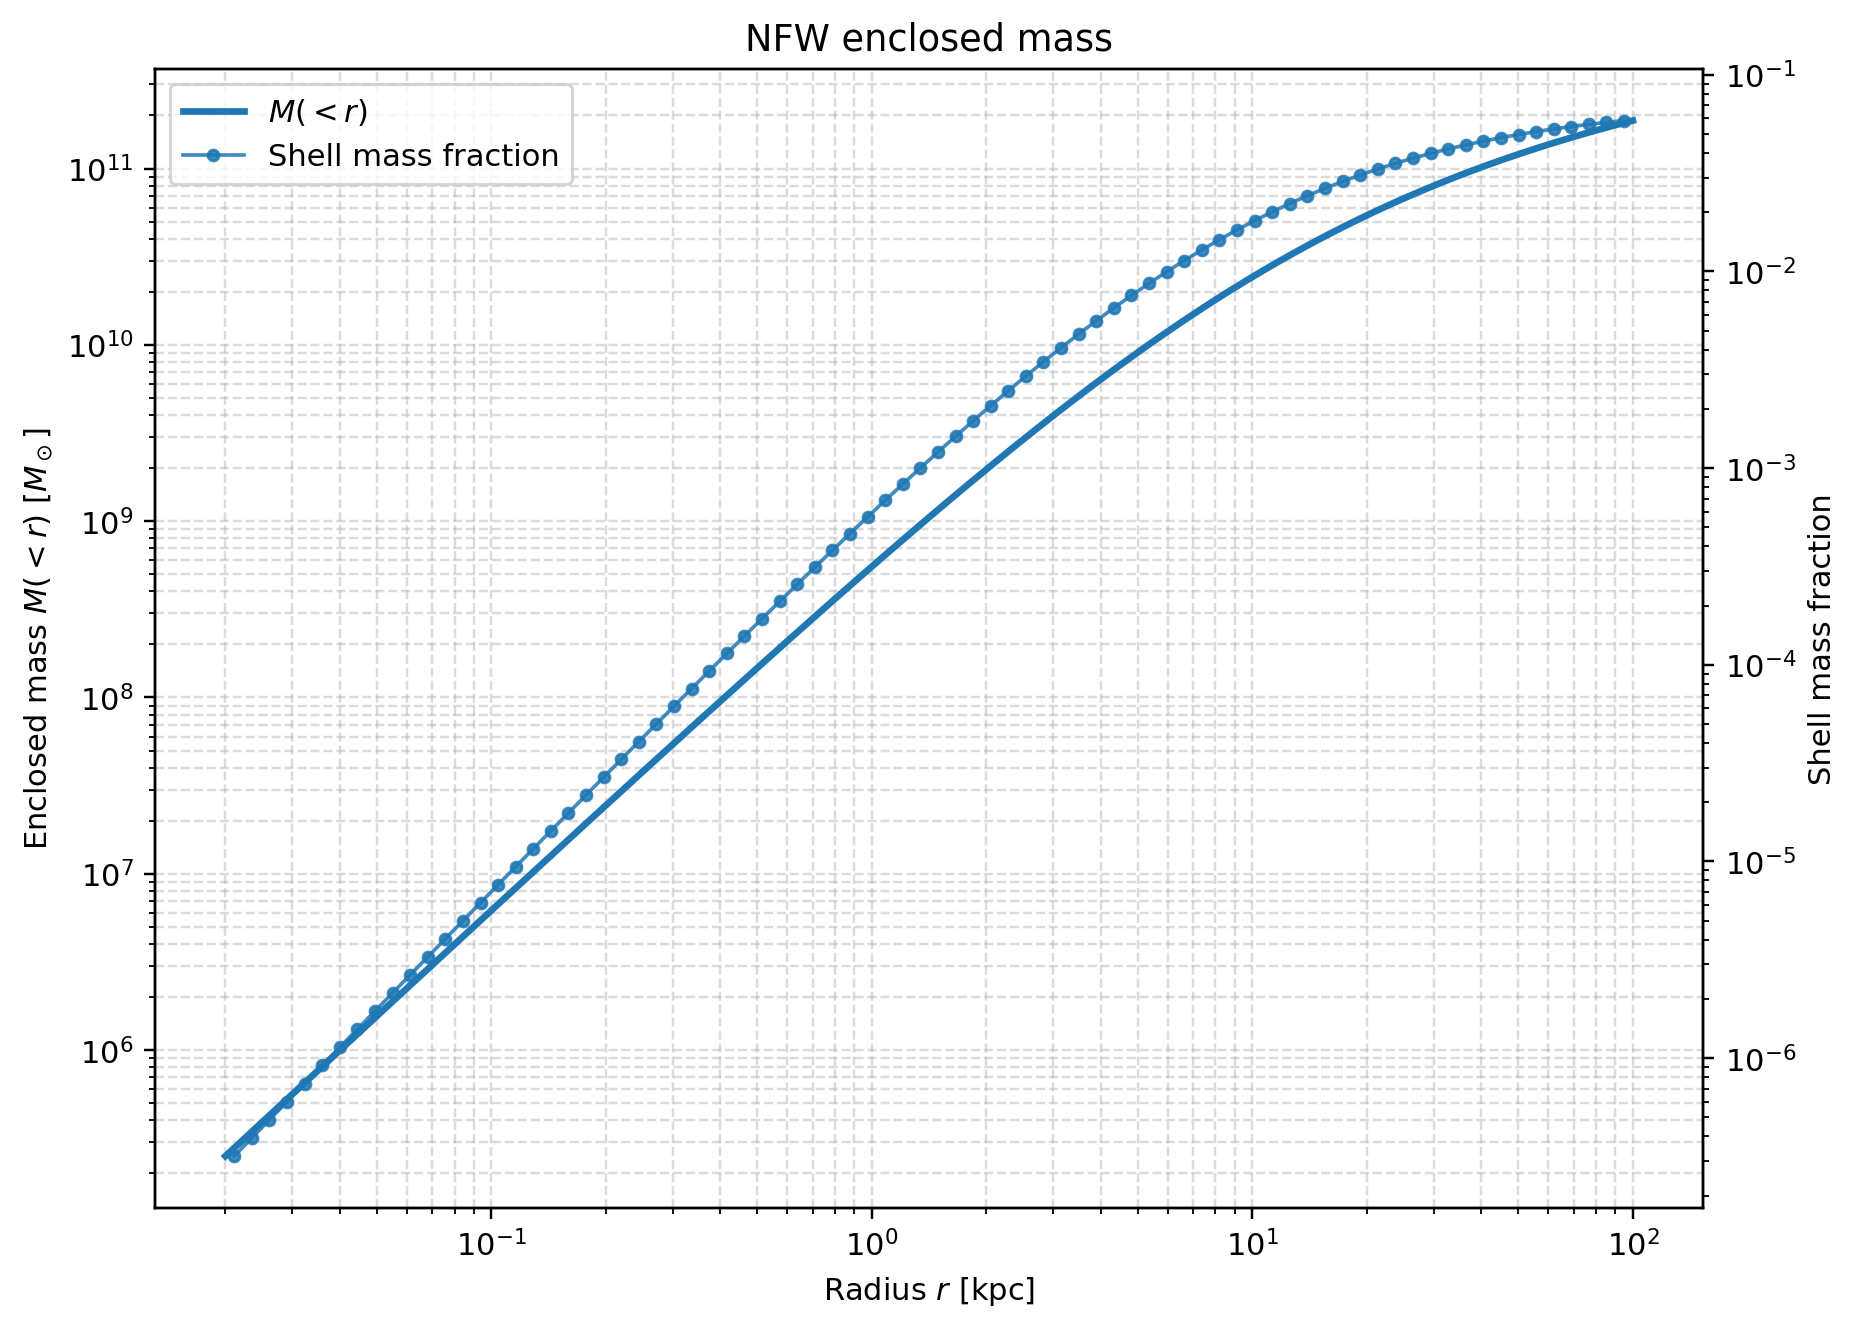
\includegraphics[width=0.85\textwidth]{content/ch5/img/01_mass_profile_and_shell_fraction.png}
	\caption{\textbf{NFW enclosed mass and shell mass fraction.} Left axis: monotonically increasing enclosed mass $M(<r)$ with radius. Right axis: shell mass fraction per logarithmic shell.}
	\label{fig:results_shell_mass}
\end{figure}

The enclosed-mass profile follows the expected NFW form: steep near the center and flattening at larger radii. Importantly, the shell mass fraction plot shows that although the inner shells contain many particles per unit volume (high density), the integrated mass grows progressively outward. Shells at radii $r > 20$ kpc contain a cumulatively significant mass fraction, establishing that the outer halo is not negligible.

Figure \ref{fig:results_shell_potential} shows the contribution of each shell to the gravitational potential at the center and the cumulative contribution from all shells outside a given radius.

\begin{figure}[H]
	\centering
	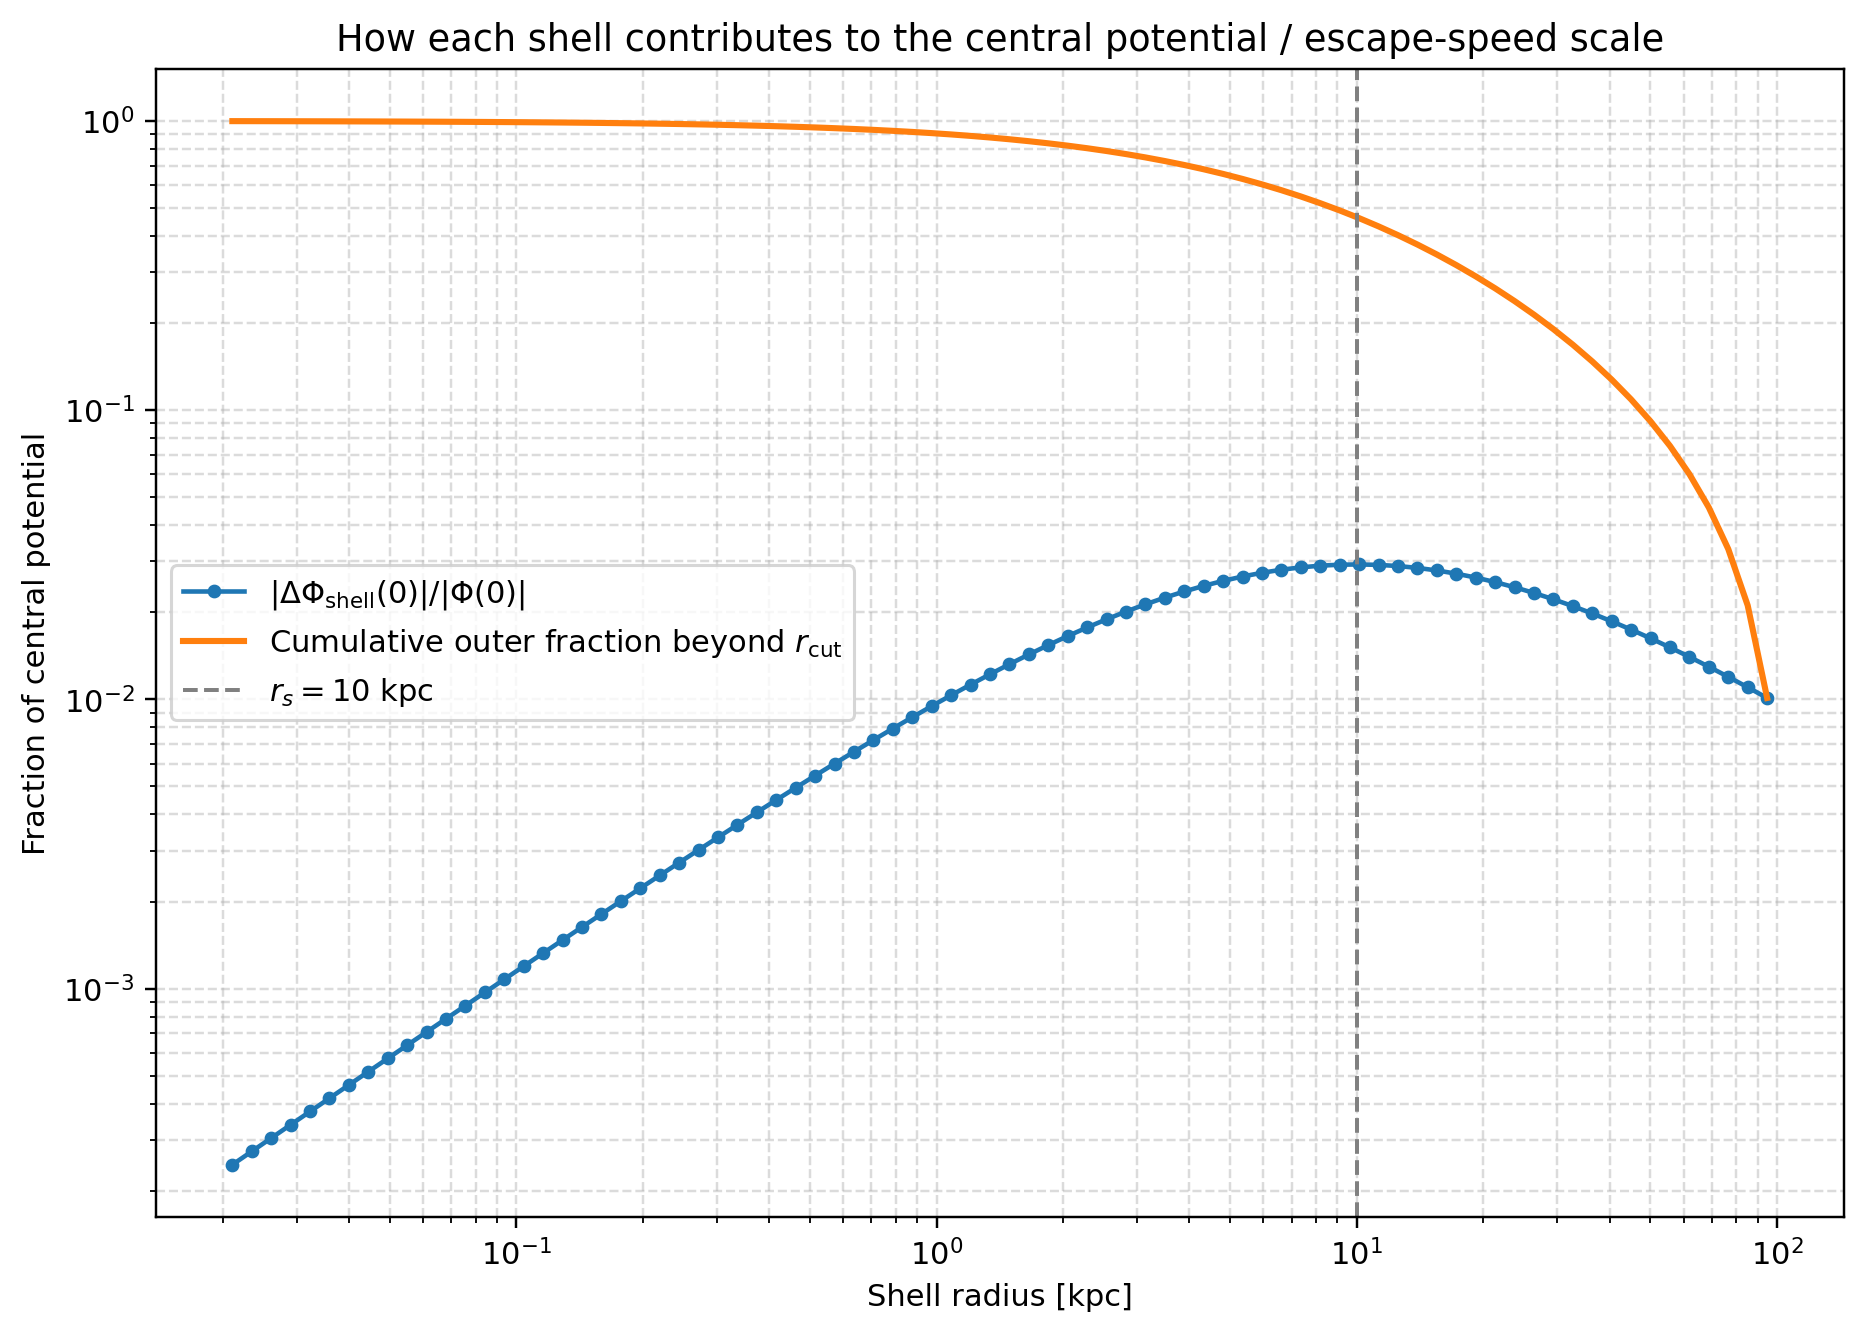
\includegraphics[width=0.85\textwidth]{content/ch5/img/02_central_potential_shell_contribution.png}
	\caption{\textbf{Shell contributions to the central potential depth.} Individual shells (blue points with error bars) contribute to the total potential depth $|\Phi(0)|$. The cumulative contribution (orange line) from all shells beyond a given radius shows that shells at radii beyond the scale radius $r_s$ still make substantial contributions to the escape-speed scale.}
	\label{fig:results_shell_potential}
\end{figure}

The key finding here is that shells well outside the center, at radii several times the scale radius, still contribute visibly to the potential depth. The fractional contribution decreases with radius but remains non-negligible up to $r \sim 3 r_s$. This result motivates the choice of cutoff radius in the hybrid model; setting $r_{\mathrm{cut}}$ too small would omit a significant part of the potential structure.

\subsection{Outer-halo influence as a function of cutoff radius}

The most critical diagnostic for the hybrid model design is the outer potential fraction. The fraction of the total potential at a given probe radius that arises from material beyond a chosen cutoff radius. Figure \ref{fig:results_shell_cutoff} shows this quantity for several probe radii as the cutoff radius is increased.

\begin{figure}[H]
	\centering
	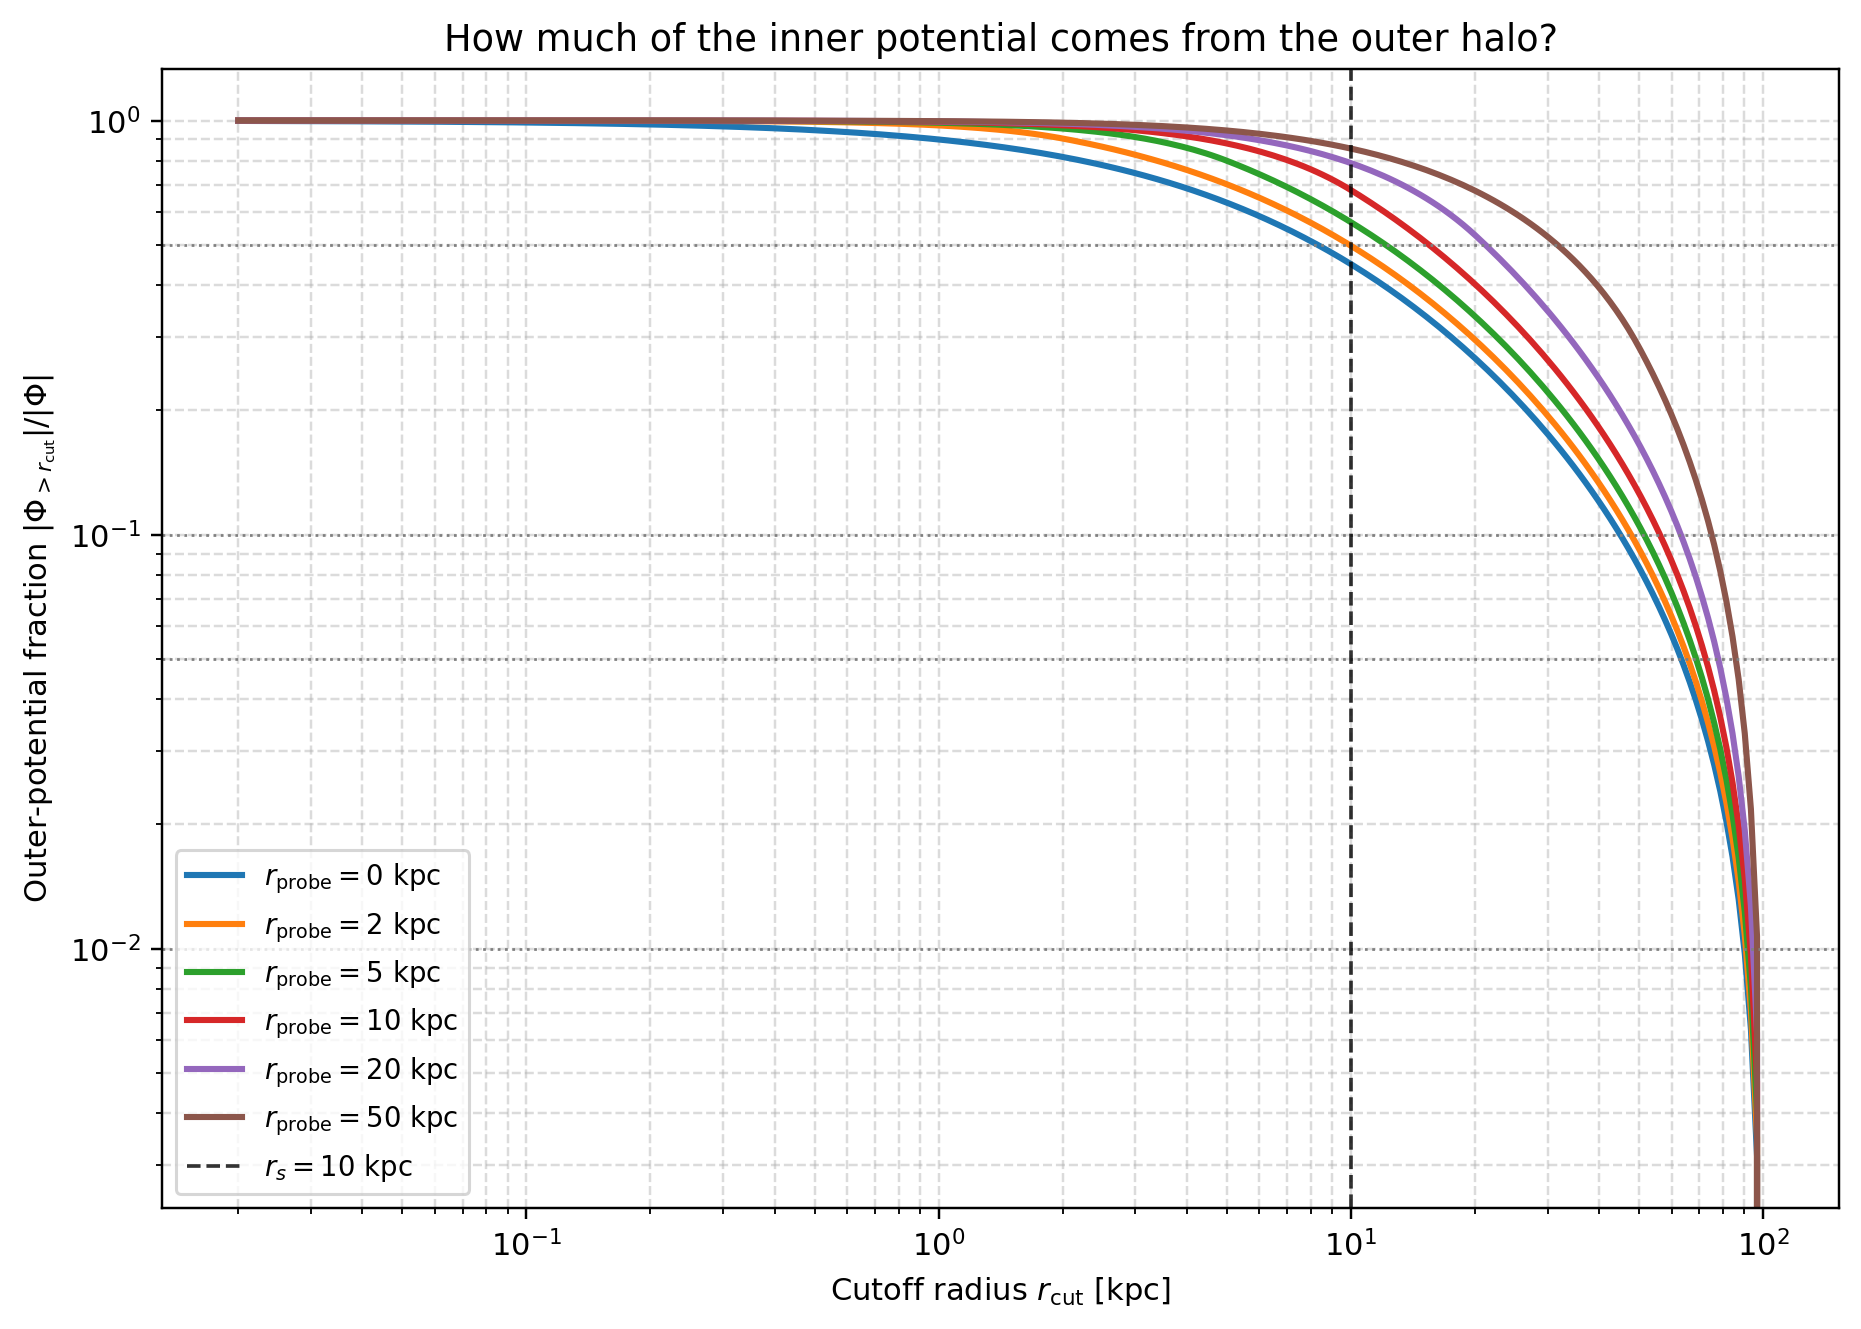
\includegraphics[width=0.85\textwidth]{content/ch5/img/03_outer_fraction_vs_cutoff.png}
	\caption{\textbf{Outer-potential fraction versus cutoff radius.} For probe radii ranging from the center to $r = 5 r_s$, the fraction of the potential originating from material beyond the cutoff radius $r_{\mathrm{cut}}$ is plotted against the cutoff. As the cutoff moves outward, the outer contribution drops sharply initially, then plateaus. For the central region ($r_{\mathrm{probe}} < r_s$), a cutoff at $r_{\mathrm{cut}} \approx 10$ kpc retains roughly 5--10\% of the potential from the outer halo; at $r_{\mathrm{cut}} \approx 30$ kpc, this drops below 1\%. Thus, if the outer halo contributes significantly to the potential at the radii of interest (e.g., $r < 1$ kpc for the central density), then the outer region must be represented accurately.}
	\label{fig:results_shell_cutoff}
\end{figure}

The curves in this figure answer the central question: how large must $r_{\mathrm{cut}}$ be to capture the essential potential structure? For the central region, a cutoff at $r_{\mathrm{cut}} = 10$ kpc retains the majority of the potential at small radii while excluding the outermost, kinematically less important material. This is a quantitative justification for the parameter choice in the numerical hybrid experiment.

\subsection{2D outer-fraction map}

Figure \ref{fig:results_shell_map} provides a compact summary of the outer-potential fraction across all combinations of probe and cutoff radii.

\begin{figure}[H]
	\centering
	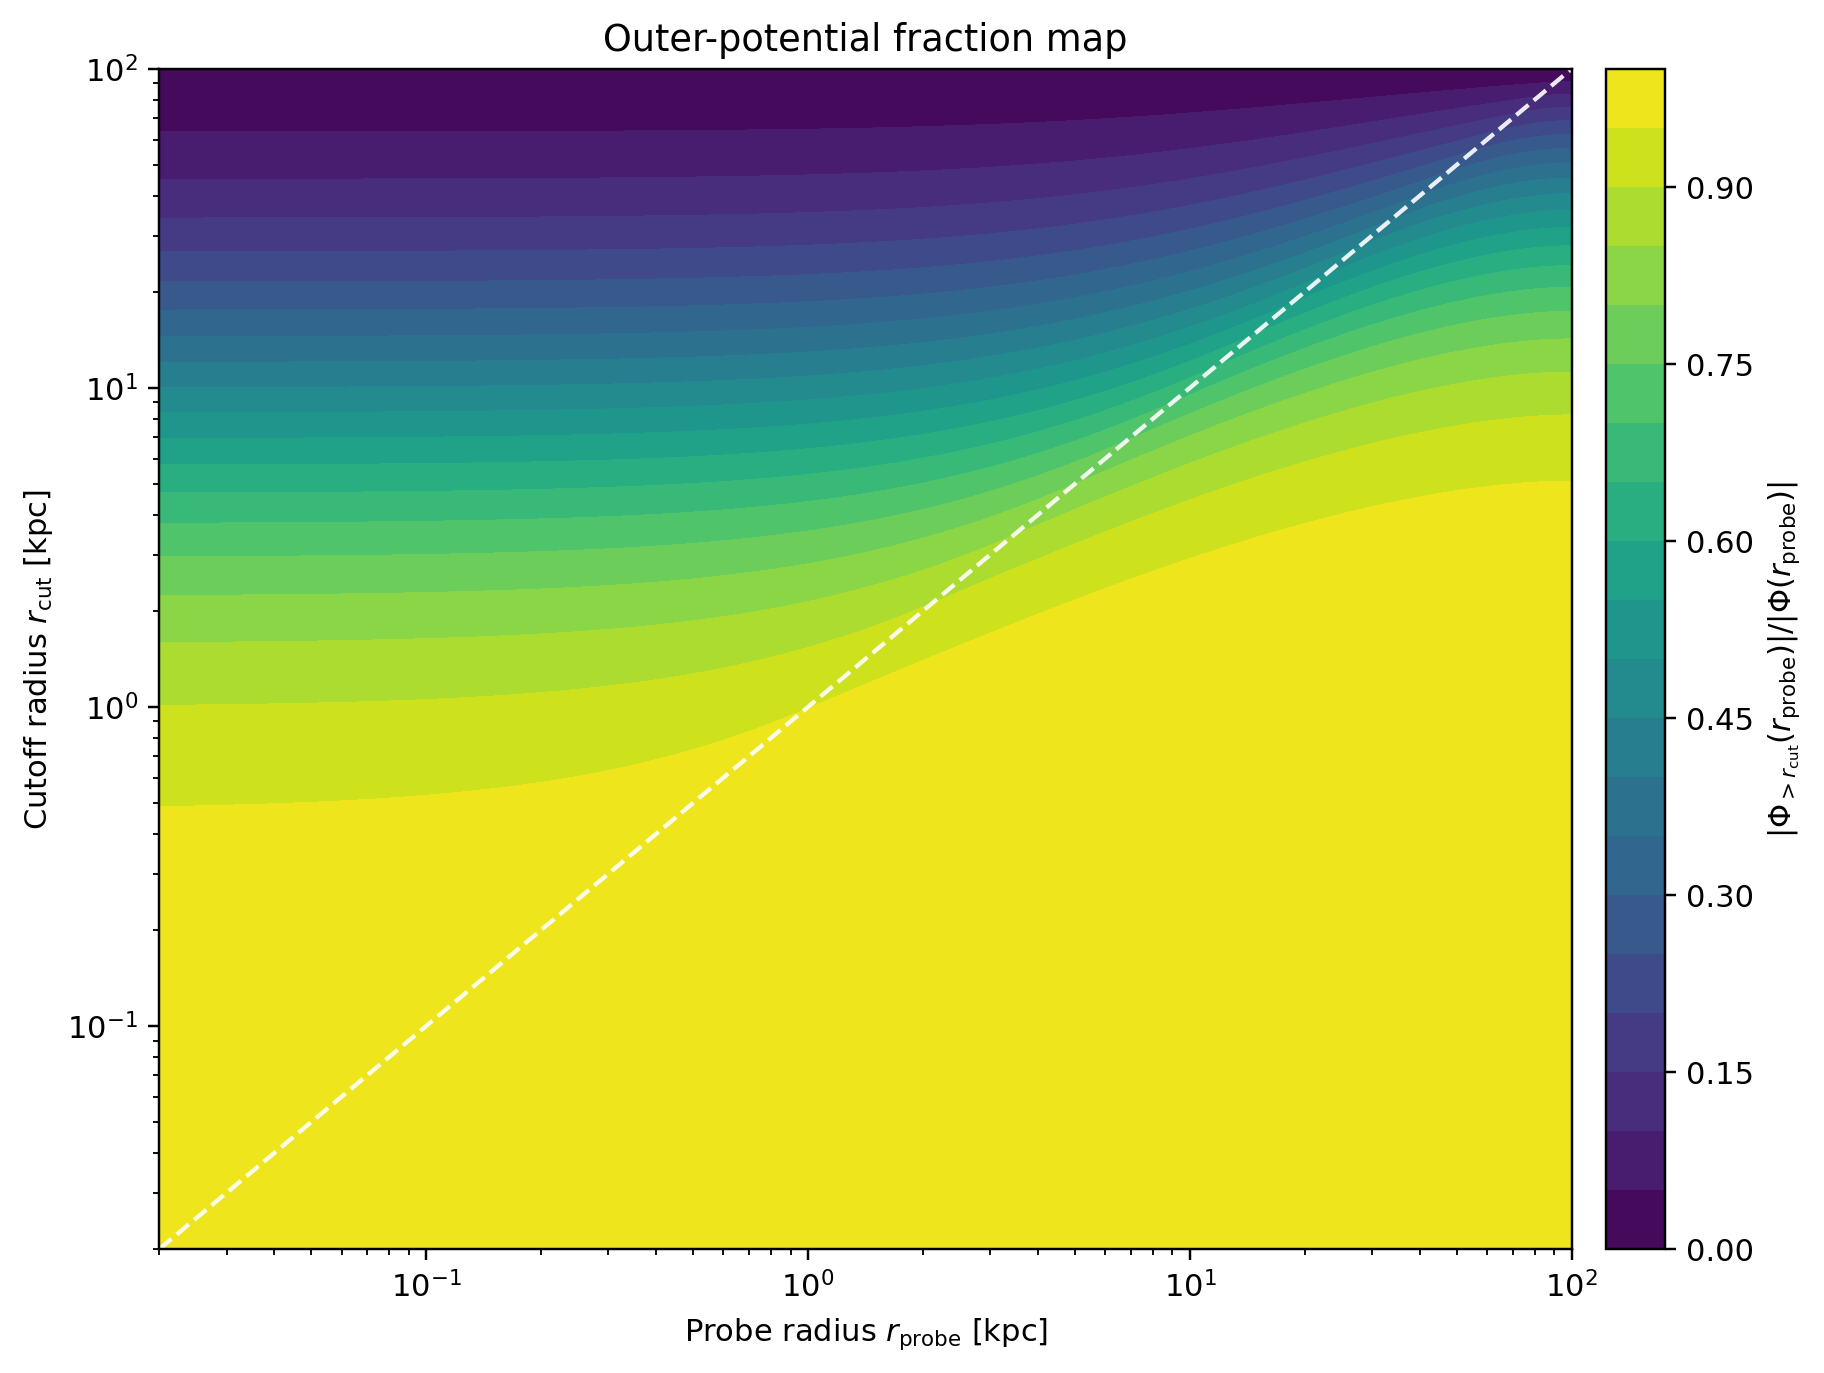
\includegraphics[width=0.85\textwidth]{content/ch5/img/04_outer_fraction_map.png}
	\caption{\textbf{2D map of the outer-potential fraction.} Rows represent probe radii; columns represent cutoff radii. The color intensity indicates the fraction of potential at a given probe radius arising from material beyond the cutoff. The transition from high (red) to low (blue) values shows the radius beyond which the outer halo becomes a small correction.}
	\label{fig:results_shell_map}
\end{figure}

The 2D map reveals the structure clearly: for small cutoff radii (lower rows), a broad range of inner probe radii feel substantial outer halo influence. As the cutoff moves outward, this influence shrinks to a narrow band near the cutoff itself.


